\documentclass{article}

\usepackage{graphicx}
\usepackage{tikz}
\usepackage{tikzsymbols}
\usetikzlibrary{calc,patterns,shapes.geometric}
\pagestyle{empty}
\usepackage[margin=0pt]{geometry}
\geometry{papersize={14in,12in}}

\def\centerarc[#1](#2)(#3:#4:#5){\draw[#1] ($(#2)+({#5*cos(#3)},{#5*sin(#3)})$) arc (#3:#4:#5);}

\begin{document}
	\begin{figure}
		\centering
		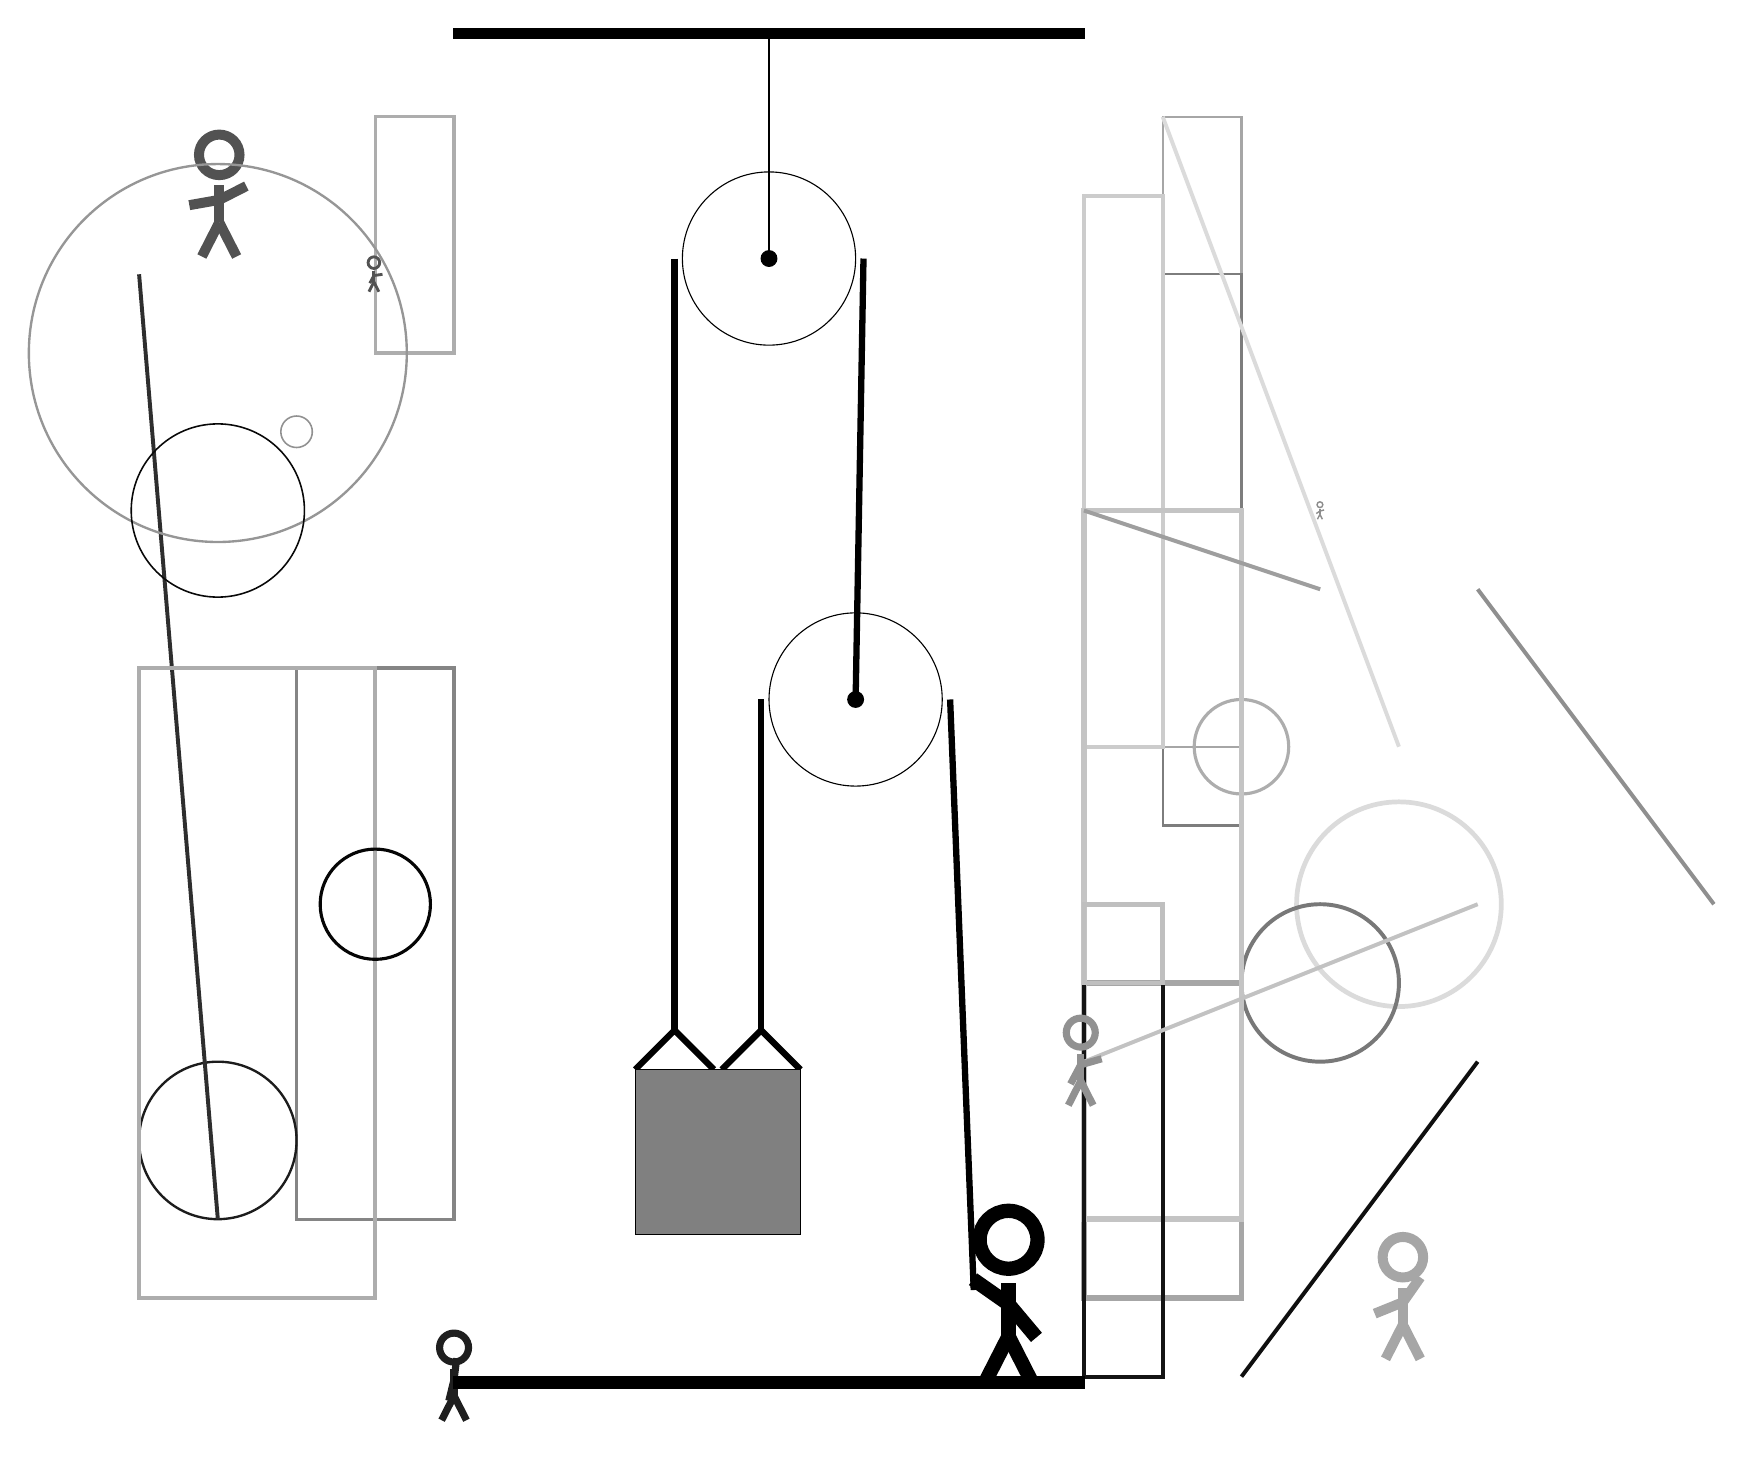
\begin{tikzpicture}
			%%%%% START %%%%%
			
			\draw[fill=black] (-2, 14) rectangle (6, 14.125);
			
			\draw (2, 11.2) circle (1.1);
			\draw[fill=black] (2, 11.2) circle (0.1);
			\draw[thick] (2, 11.2) -- (2, 14);
			
			\draw (3.1, 5.6) circle (1.1);
			\draw[fill=black] (3.1, 5.6) circle (0.1);
			
			\draw[line width=0.7mm, color=black!35] (6, -2) rectangle (8, 2);
			
			\node[line width=0.4mm, color=black!45] at (9, 8) {\Strichmaxerl[1][33][16]};
			\draw [line width=0.6mm, color=black!14](10, 3) circle (1.3);
			\draw[line width=0.3mm, color=black!35] (7, 13) rectangle (8, 5);
			\draw [line width=0.2mm, color=black!16](9, 2) circle (1.0);
			\draw[line width=0.5mm, color=black!44](11, 7) -- (14, 3);
			\draw[line width=0.3mm, color=black!51] (7, 4) rectangle (8, 11);
			
			\draw [line width=0.5mm, color=black!53](9, 2) circle (1.0);
			\draw[line width=0.4mm, color=black!32] (-3, 10) rectangle (-2, 13);
			\draw [line width=0.2mm, color=black!43](-4, 9) circle (0.2);
			\draw [line width=0.4mm, color=black!32](8, 5) circle (0.6);
			
			\draw[line width=0.4mm, color=black!48] (-4, 6) rectangle (-2, -1);
			\draw[line width=0.5mm, color=black!20] (7, 5) rectangle (6, 12);
			
			\draw [line width=0.3mm, color=black!89](-5, 0) circle (1.0);
			\node[line width=0.2mm, color=black!68] at (-3, 11) {\Strichmaxerl[2][62][8]};
			\draw[line width=0.5mm, color=black!82](-6, 11) -- (-5, -1);
			
			\node[line width=0.6mm, color=black!68] at (-5, 12) {\Strichmaxerl[7][10][27]};
			
			\draw [line width=0.3mm, color=black!41](-5, 10) circle (2.4);
			\draw[line width=0.7mm, color=black!23] (8, -1) rectangle (6, 8);
			\node[line width=0.2mm, color=black!35] at (10, -2) {\Strichmaxerl[7][22][55]};
			\draw[line width=0.5mm, color=black!32] (-3, -2) rectangle (-6, 6);
			
			\draw[line width=0.5mm, color=black!92] (7, -3) rectangle (6, 2);
			\draw [line width=0.2mm, color=black!97](-5, 8) circle (1.1);
			\draw[line width=0.5mm, color=black!38](9, 7) -- (6, 8);
			\draw[line width=0.6mm, color=black!25] (7, 3) rectangle (6, 2);
			
			\draw [line width=0.4mm, color=black!98](-3, 3) circle (0.7);
			
			\draw[line width=0.5mm, color=black!94](11, 1) -- (8, -3);
			\draw[line width=0.5mm, color=black!24](11, 3) -- (6, 1);
			\node[line width=0.2mm, color=black!43] at (6, 1) {\Strichmaxerl[5][62][16]};
			
			\draw[line width=0.5mm, color=black!14](10, 5) -- (7, 13);
			\node[line width=0.2mm, color=black!88] at (-2, -3) {\Strichmaxerl[5][76][83]};
			
			\draw[line width = 0.8mm]  (0.3, 0.9) -- (0.8, 1.4) -- (1.3, 0.9);
			\draw[line width = 0.8mm]  (1.4, 0.9) -- (1.9, 1.4) -- (2.4, 0.9);
			\draw[fill=black!50] (0.3, 0.9) rectangle (2.4, -1.2);
			
			\draw[line width = 0.8mm] (0.8, 11.2) -- (0.8, 1.4);
			\centerarc[line width = 0.8mm](2, 11.2)(0:180:1.2000000000000002);
			\draw[line width = 0.8mm] (3.2, 11.2) -- (3.1, 5.6);
			\draw[line width = 0.8mm] (1.9, 5.6) -- (1.9, 1.4);
			\centerarc[line width = 0.8mm](3.1, 5.6)(0:180:1.2000000000000002);
			\draw[line width = 0.8mm] (4.3, 5.6) -- (4.6, -1.9);
			
			\node at (5, -2) {\Strichmaxerl[10][-35][-50]};
			
			\draw[fill=black] (-2, -3) rectangle (6, -3.15);
			
			%%%%% END %%%%%
		\end{tikzpicture}
	\end{figure}	
\end{document}